%% Template by Chloé Rouyer, Aimed for theses written at DIKU. 
%% This templaate is aimed to be easy to use and highly customizable. 
%% Contact if questions at chloerouyer.ml@gmail.com

%% Inspired from the template of Alex Jørgensen
%% https://www.overleaf.com/latex/templates/thesis-and-project-ucph/jnvpqdzrhrzr

%%%%% General Structure of the template %%%%%

\documentclass[12pt, oneside]{book} 
% The oneside option ensures that all pages are similar. the default option 'twosides' distinguishes between left and right pages.
\usepackage{KUstyle}
\usepackage[toc,page]{appendix}
%% If you want to modify from the default margins
% \usepackage[left= 1.1in, right = 1.1in, top = 1.5in, bottom = 1.5in]{geometry} % Set the margins
% \usepackage{layouts} % Use in combination with the command %

%%%% Personal setup %%%%%

%% bibtex Important package to use full citations: bibentry
% \usepackage[super]{natbib}
\usepackage[numbers]{natbib}
% \usepackage{cite}
\usepackage{bibentry}
\newcommand\citeAY[1]{\citeauthor{#1} (\citeyear{#1})}
% \usepackage[autocite=superscript]{biblatex}
% \usepackage{biblatex}
\nobibliography*

\bibliographystyle{plainnat}

\definecolor{kurød}{rgb}{0.565, 0.102, 0.118}

\definecolor{PMGcolor}{rgb}{0.0, 0.690, 0.314}
\definecolor{VFcolor}{rgb}{0.0, 0.439, 0.753}
% \definecolor{GBcolor}{rgb}{0.565, 0.102, 0.118}

\hypersetup{colorlinks=true, urlcolor=kurød, citecolor = kurød, linkcolor = kurød}
\usepackage{float}
% \usepackage{caption}
\usepackage{subcaption}
\usepackage{graphicx}
\usepackage{outlines}
\usepackage{amsmath}
\setlength\parindent{0pt}
\usepackage[font={small},labelfont=bf, format = hang,indention=-1.5cm]{caption}
\usepackage{wrapfig}
\usepackage{etoc}

% Reset indentation specifically for subfigures
\captionsetup[subfigure]{format=hang, labelfont=bf, indention=-0.3cm}


\newcommand{\todo}[1]{\textcolor{purple}{\textbf{TODO: #1}}}
\newcommand{\note}[1]{\textcolor{orange}{\textbf{Note: #1}}}
\newcommand{\reph}[0]{\textcolor{red}{\textbf{Rephrase!}}}
\interfootnotelinepenalty=10000



\newcommand{\vf}[1]{\textcolor{VFcolor}{\textbf{#1}}}
\newcommand{\gb}[1]{\textcolor{kurød}{\textbf{#1}}}
\newcommand{\pmg}[1]{\textcolor{PMGcolor}{\textbf{#1}}}
\newcommand{\cephalic}[1]{\textcolor{yellow}{\textbf{#1}}}


\definecolor{lightblue}{rgb}{0.357,0.592,0.863}
\newcommand{\lightblue}[1]{\textcolor{lightblue}{\textbf{#1}}}

\definecolor{lightred}{rgb}{0.745,0.372,0.345}
\newcommand{\lightred}[1]{\textcolor{lightred}{\textbf{#1}}}

\definecolor{lightyellow}{rgb}{0.886,0.741,0.172}
\newcommand{\lightyellow}[1]{\textcolor{lightyellow}{\textbf{#1}}}

\definecolor{lightpurple}{rgb}{0.4,0.373,0.592}
\newcommand{\lightpurple}[1]{\textcolor{lightpurple}{\textbf{#1}}}



\usepackage{listings}  % For presenting code 
\lstdefinestyle{mystyle}{
  language=Python,
  basicstyle=\ttfamily\footnotesize,
  backgroundcolor=\color[HTML]{F7F7F7},
  rulecolor=\color[HTML]{EEEEEE},
  identifierstyle=\color[HTML]{24292E},
  emphstyle=\color[HTML]{005CC5},
  keywordstyle=\color[HTML]{D73A49},
  commentstyle=\color[HTML]{6A737D},
  stringstyle=\color[HTML]{032F62},
  emph={@property,self,range,True,False},
  morekeywords={super,with,as,lambda},
  literate=%
    {+}{{{\color[HTML]{D73A49}+}}}1
    {-}{{{\color[HTML]{D73A49}-}}}1
    {*}{{{\color[HTML]{D73A49}*}}}1
    {/}{{{\color[HTML]{D73A49}/}}}1
    {=}{{{\color[HTML]{D73A49}=}}}1
    {/=}{{{\color[HTML]{D73A49}=}}}1,
  breakatwhitespace=false,
  breaklines=true,
  captionpos=b,
  keepspaces=true,
  numbers=none,
  showspaces=false,
  showstringspaces=false,
  showtabs=false,
  tabsize=4,
  frame=single,
}
\lstset{style=mystyle}

% \usepackage[font={small, sl},labelfont=bf]{caption}
% \newcommand{}[]{}

%% You can put all packages and personalized commands in the following document.
% IMPORTANT! In order for the document to compile, one needs to use XeLaTeX or LuaLaTeX as compiler. This can be done in  Overleaf by Menu -> Settings -> Compiler -> Choose XeLaTeX/LuaLaTeX

%% These are the packages and commands that I used, feel free to remove and edit them.

%% Set the path for your images. Remember to edit all your includegrpahics to the correct location.
 \graphicspath{ {images/} }

%% Suggested Commands %%

%% Personal favourite command if you want to number a single line in a series of equations. Use an align* environement and use \numberthis specifically on the line that you want to number rather than using an align environement and \notag on every line you don't want to number.  
\newcommand\numberthis{\addtocounter{equation}{1}\tag{\theequation}}

%% If you have Dutch names in your references 
\DeclareRobustCommand{\VAN}[3]{#2} % proper Dutch 'van/de' capitalisation

%% If you want your theorems to include the Chapter numbers in the nmumbering
\usepackage{amsthm} %P ackage that gives the theorems environment

\newtheorem{prop}{Proposition}[chapter]
\newtheorem*{prop*}{Proposition}
\newtheorem{example}{Example}[chapter]
\newtheorem{proof_sketch}{Sketch of the Proof}[chapter]
\newtheorem{theorem}{Theorem}[chapter]
\newtheorem{lemma}{Lemma}[chapter]
\newtheorem*{lemma*}{Lemma}
\newtheorem{remark}{Remark}[chapter]
\newtheorem{definition}{Definition}[chapter]
\newtheorem{corollary}{Corollary}[chapter]
\newtheorem{notation}{Notation}[chapter]


%% Other packages I typically use. 

% \usepackage{geometry}
% \usepackage{setspace} % Package for linespacing
% \usepackage{tabularx} % Package for table
% \usepackage{fontspec}

% \usepackage[T1]{fontenc}    % use 8-bit T1 fonts
% \usepackage{url}            % simple URL typesetting
% \usepackage{booktabs}       % professional-quality tables
% \usepackage{amsfonts}       % blackboard math symbols
% \usepackage{nicefrac}       % compact symbols for 1/2, etc.


% \usepackage{xcolor}         % colors
% \usepackage{dsfont}
% \usepackage{bm}
% \usepackage{mathtools}
% \usepackage{cleveref}
% \usepackage{amsmath}
% \usepackage{amssymb}
% \usepackage{xifthen}
% \usepackage[ruled]{algorithm2e}
% \usepackage{algorithmic}


%%%% Template Related Setup %%%%%

%%% Front Page %%%
\ptype{Masters Thesis}

\fpimage{evangelion.png}
% \fpimage{template/frontpage.png}
\author{Jakob Hallundbæk Schauser}
\title{Emergence and Mesoscopy:\\ Drosophila Gastrulation In Silico}
\subtitle{Uncovering macroscopic morphogenesis\\ from simulating microscopic biophysics}
\advisor{Supervisor: Ala Trusina}
\date{October 2024}
%% This sentence is needed for PhD theses, but it can be replaced by the date for other projects.

\renewcommand{\contentsname}{Table of Contents}

%%% Report parameters %%%

%% Table of contents %%
% Set table of contents depth:  {1} only includes sections, {2} also includes subsections
 \setcounter{tocdepth}{1}

% Specific entries can be added manually with a command such as: 
% \addcontentsline{toc}{section}{[Title of Section]}  %Use section or chapter to decide how this extra element should be displayed
 
% remove the dots in the table of contents
%  \makeatletter
% \renewcommand\@dotsep{280}   % default value 4.5
% \makeatother

%% Section Numbering within the chapters %%
% number sections until subsubsections (set to 2 to number until subsections, and to 4 to number paragraphs)
 \setcounter{secnumdepth}{3}
 
%% Set Chapter title in header %% 
\usepackage{titlesec}
\usepackage{fancyhdr}

% plain style so that the header does not appear in the abstract
\fancypagestyle{plain}{         
\fancyhf{}
\fancyfoot[C]{\thepage}}%

% new style for the mainmatter with the line under the title
\renewcommand{\headrulewidth}{0pt}
\renewcommand{\chaptermark}[1]{\markboth{#1}{}}
\newcommand\mymainpagestyle{%
\fancyhf{}      
\fancyhead[L]{\nouppercase{\footnotesize{\chaptername~ \thechapter~ |~ \leftmark}} \renewcommand{\headrulewidth}{0.4pt} \headrule \renewcommand{\headrulewidth}{0pt}}
\setlength{\headheight}{25pt}
\fancyfoot[C]{\thepage}
}

%% alternate style for the mainmatter without the line under the title
% \renewcommand{\headrulewidth}{0pt}
% \renewcommand{\chaptermark}[1]{\markboth{#1}{}}
% \newcommand\mymainpagestyle{%
% \fancyhf{}      
% \fancyhead[L]{\nouppercase{\footnotesize{\chaptername~ \thechapter~ |~ \leftmark}} }
% \setlength{\headheight}{25pt}
% \fancyfoot[C]{\thepage}
% }

%% Note: if you want to use a different running title in the header, you can use the following structure when giving your title:
% \chapter{Long chapter title}
% \chaptermark{Short chapter title}


%%%%% Main %%%%%

\begin{document}

% \pagevalues  % If you are using the package layouts and want to get the current layout margin values so you can tune them. They are displayed on the first page if you activate this option. Remember to uncomment the \usepackage{layouts} at the beginning of this document. 


%%%% Introduction %%%%
\maketitle
\frontmatter % to get a different numbering of the frontmatter and mainmatter.
\pagestyle{plain} % not to get a header in the introduction pages

\newpage \ \\\\\\\\\\\\\textit{"Art and technology have been trying for decades, but in the world of physics, not a lot of complexity is needed for something akin to life to emerge"} \\- Goodiepal in the 11th hour% (16:40) \newpage % to skip a page 

% The Abstract, Danish Abstract and Acknowledgements are not numbered here but still appear in the table of contents.
\section*{Abstract}
\label{sec:abstract}
\addcontentsline{toc}{section}{Abstract} 

% \newpage
% \section*{Resumé}
% \label{sec:resume}
% \addcontentsline{toc}{section}{Resumé}

\newpage
\section*{Acknowledgements}
\label{sec:acks}
\addcontentsline{toc}{section}{Acknowledgements}


\newpage
\tableofcontents
\newpage


%%%% Introduction %%%%
\mainmatter 
\mymainpagestyle{} % to get a header in the rest of the chapters (excpet the first page of the chapter)

\chapter{Introduction}
\label{chap:intro}
In 1952, two years before his untimely death, Alan Turing wrote an article called
\textit{The chemical basis of morphogenesis}.\cite{turing52the} In it, he predicted that off-equilibrium chemicals, with . He coined the term morphogens thereby cementing .\footnote{This paper was written \textit{one year} before the discovery of DNA and still use the word "gene" as its old "functional unit of heredity"} Much like cellular automata, 



It is suggested that a system of chemical substances, called morphogens, reacting together and diffusing through a tissue, is adequate to account for the main phenomena of morphogenesis through the emergence of genetic patterning.

When studying the interplay between morphogens and morphogenesis, no other organism has been studied as much as Drosophila Melongaster (the common fruit fly among friends).



\section{Why do we care about emergence?}
Leptin (1999) Review

From morphogen to morphogenesis and back
\section{Why do we care about Morphogenesis}
Plato used the words \textit{form} and \textit{idea} interchangeably

Morphogenesis involve coordination

All cells use the same array of actions to achieve wildly different results.  

"Morphogenesis in embryogenesis is one of the most interesting and rich sources of challenging problems in biomechanics."

As mentioned earlier, the  from the genetic makeup, local cell-neighborhood, global environment and maternal effects, all have an influence in a way YY many factors seems to corroborate successful embryogenesis. 

Combining the (1) limited set of actions (2) Timing/coordination (3)information sharing/retention (4) something else, makes the subject ripe for us(?):

Simulating these individual parts grants us the possibility for a potential bottoms-up understanding of the complete/whole.



\section{Why do we care about Modeling}
Main idea: Using a simple model, can complex, staggered morphological events emerge. And can such a simple model be used for making predictions?
Main idea2: How much is information is single-cell level and how much is BC, etc.

% place yourintroduction there

% place your chapters there
\chapter{Theory}
\label{chap:theo}
Before getting to all the fun graphs, we will need to introduce some concepts, so you\footnote{yes, \textit{you} specifically} can follow along while keeping me somewhat consistent with the literature:

\begin{enumerate}
    \item Upper/Lower $\rightarrow$ Dorsal/Ventral
    \item Front/Back  $\rightarrow$ Anterior/Posterior
    \item   $\rightarrow$
\end{enumerate}

Whenever an diagram or image of the egg is show, the Anterior side is pointing to the left.

\section{Broken Symmetries and Genetic Patterning}
% \section{Everything}
\label{sec:theory-polarity}
\subsection{Broken Symmetries}

Almost all animals [Citation needed] start as a single, isotropic sphere of epithelial cells. At one point, this ball will 'turn in on itself' and begin developing the basis for organogenesis. This process is called gastrulation. As animals are not spherically symmetric\footnote{except for your mom}, a number of symmetries need to be broken. 

In drosophila, after the first rounds of mitosis, the cells migrate to line the inside of their egg. This allows their surfaces form distinct "outside" and "inside" domains. Through preferential adhesion\footnote{explain  preferential adhesion} based on their individual surface orientation, the cells can maintain the shell-form, thereby giving rise to the well-defined Inside-Outisde polarity. In biology this is known as Apical-Basal polarity (AB-polarity from here on) and is seen in almost every multicellular system. 

We will quickly outline the main morphological features of the gastrulation cycle of the embryo:
\begin{outline}
    \1 Posterior Midgut (PMG)
    \1 Anterior Midgut (AMG)
    \1 Ventral Furrow
    \1 Dorsal Transverse Furrows
    \1 Cephalic Furrow
    \1 Germ Band
\end{outline}

\begin{figure}[H]
    \centering
    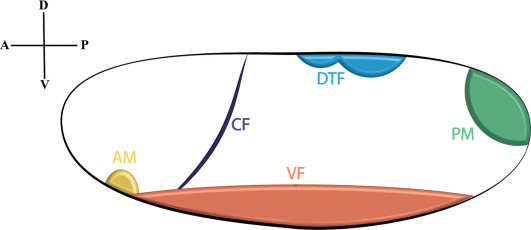
\includegraphics[width = 0.7\linewidth]{chapters/Theory/figures/morphogenic_events.jpg}
    \caption{Summary of the morphogenetic events mapped onto the blastoderm stage embryo. Taken from \cite{gheisari2020gastrulation}. The colored parts are generally seen to be the morphogenetically active during the early part of the embryogenesis}
    \label{fig:enter-label}
\end{figure}



Diffusion based concentration gradients along with the aforementioned polarities allow for spatially complex, precise and robust macro scale morphology changes.

\subsection{Genetic Patterning}
\label{sec:gen_patterns}
All multicellular organisms, will YYY need to go from the simple single cell to forming the complex body plans we all know and love. This complicated interplay between cells will needs organization. Again, for humans and fruit fly alike, this is done via genetic patterning.\cite{veraksa2000developmental}

Thinking about this it top-down is inaccurate.


% Now, to shake it up, \textit{Twist} \& \textit{Snail}, which might remind you of the beetles,\footnote{The species \textit{Tribozium} for example\cite{sommer1994expression}} are vital for the early development of a surviving fruit fly.


During the development of our model, the data and resources at \url{https://shiny.mdc-berlin.de/DVEX/} have been absolutely vital.

TODO: Maybe explain data-processing?

This allowed us making maps. Where we initially defined areas of interes after hand-drawn cell-fate maps, we can now specify boundaries between cell types on the unperturbed morphology using interactions between maternal gradients. A selection fo some of the most vital morphogens can be seen in tabek \ref{tab:morphogens} and in Figure \ref{fig:MorphogenMap} their concentrations can be seen as mapped onto our virtual blastoderm.


\begin{table}[H]
\begin{tabular}{lll}
 \begin{tabular}[c]{@{}l@{}}Genetically patterned \\ transcription factor proteins\end{tabular} & Location at gastrulation & Vital for development of \\ \hline
 Twist \& Snail                                                                                 & Ventral                  & Mesoderm                 \\
Huckebein \& Tailless                                                                          & Posterior                & Endoderm (Midgut)   \\

 Runt \& Even skipped & Germ Band & All of the above\\
Buttonhead \& Even skipped  & Cephalic furrow & Chephalic furrow\\

\end{tabular}
    \caption{The most important morphogens and their simplified reason of significance}
    \label{tab:morphogens}
\end{table}


\noindent

\begin{figure}[H]
    \centering
    \makebox[\linewidth]{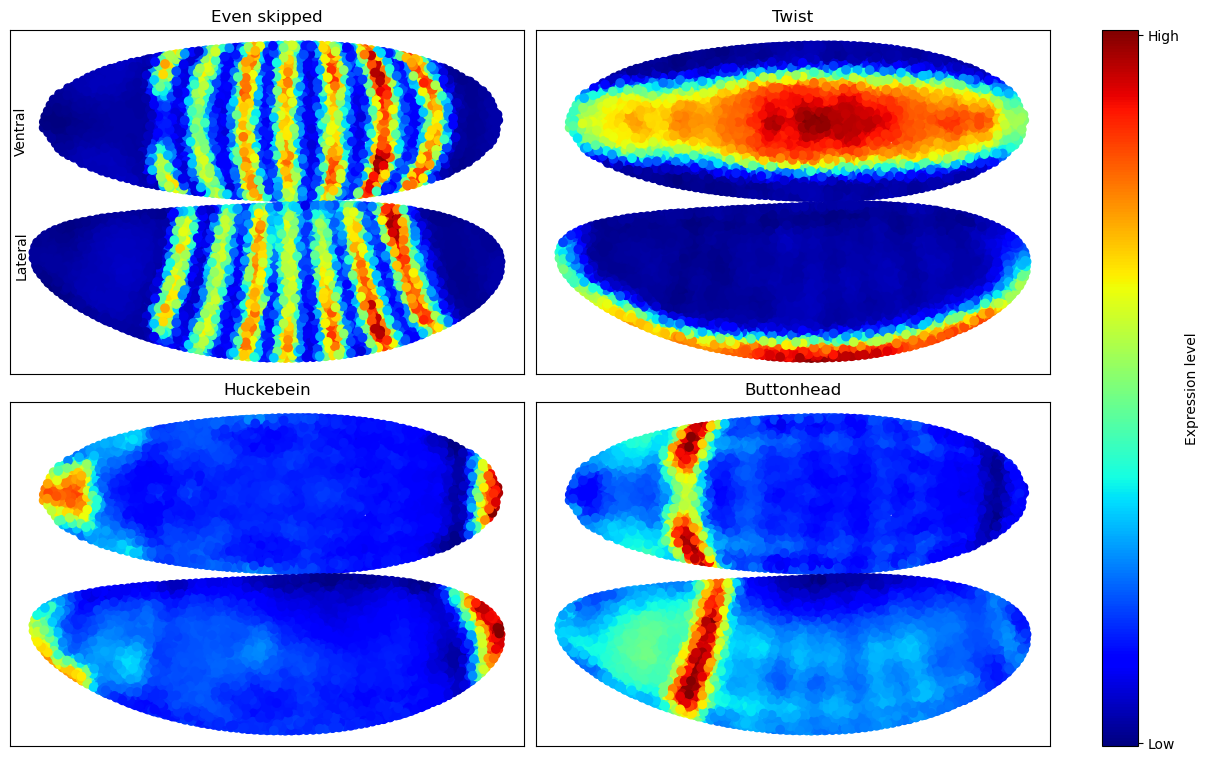
\includegraphics[width=1.2\linewidth]{chapters/Theory/figures/patterning.png}}
    \caption{The data extracted from \url{https://shiny.mdc-berlin.de/DVEX/} as projected onto our embryo. A clear attest to the remarkable and stable pattern formation Turing predicted chemicals gradients capable of producing.}
    \label{fig:MorphogenMap}
\end{figure}

Importantly, the interaction between the morphogens and the mechanical deformations go both ways. It has been shown (J. Schauser et al) that a mechanical stimulus can trigger a chemical signal, thereby reinducing patterning in a feedback loop. This is called mechanotransduction and is believed to be vital in stable PCP-orientation. [citation needed]


\textbf{Important:}
The PCP has been shown to be gradient of striping


\section{How cells move}

In general, most of the global large-scale cell migration seen during development of multicellular organisms stem from a handful of seemingly simple\footnote{albeit still not well understood} active single-cell actions.\cite{walck2014cell}\\
The cells internal structure is called the cytoskeleton with internal \textit{motor proteins} responsible for keeping and changing the cells shape.

The motion we will be looking at, are of a type that is fundamentally different from Chemotaxis, with cells reacting to a local chemical concentration but not moving along a gradient [citation needed]. The global changes in physical structure we will be exploring all arise from cell actions with little to no discernible individual movement.


When we talk about the individual cells, this is a simplification. As can be seen on Figure \ref{fig:mysosinMeshwork}, the cells stay interconnected using membrane tethers connecting local neighborhoods. 

\begin{figure}[H]
    \centering
    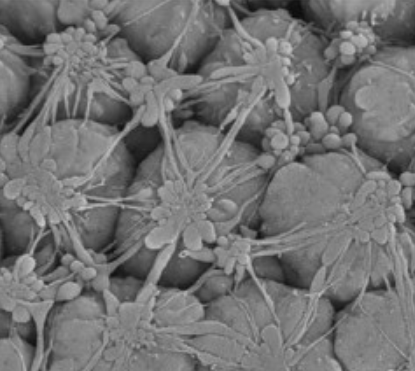
\includegraphics[width=0.6\linewidth]{chapters/Theory/figures/EM_constricting_proteins.png}
    \caption{Electron microscopy of Myosin II meshwork at ventral side. Taken from \cite{martin2010integration}}
    \label{fig:mysosinMeshwork}
\end{figure}

In Drosophila gastrulation, the role of these 'driving effects' are surprisingly under-understood with no paper claiming YYY with certainty.\footnote{This very much comes down to the fact, that experiments with living, moving cells are inherently intractable/hard} Here is a list of the fundamental single-cell active forces that is undeniably happening, even if not essential for the final outcome:\footnote{As nature is remarkably resilient, there is clear and definite evidence of one action overtaking when another fails to deliver. \textbf{Rewrite} This will be expanded upon in Section \ref{sec:mutantNoGB}} 

\subsection{Convergent Extension}
For elongating the germ band Convergent Extension seems to be the main proprietor of movement. Consisting of asymmetric cellular intercolations, tissue can change shape without the individual constituents looking any different.  

\begin{figure}[H]
    \centering
    \begin{subfigure}{0.45\linewidth}
        \centering
    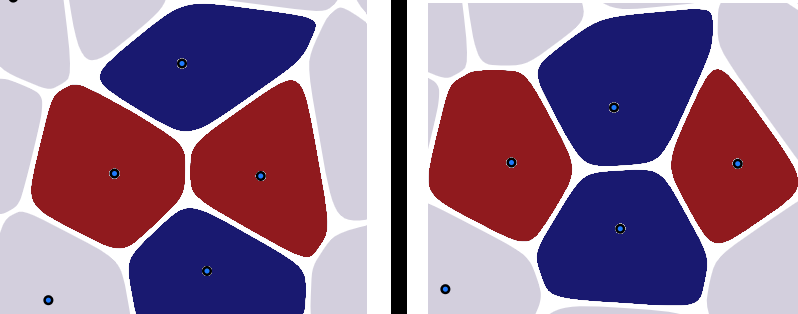
\includegraphics[width=\linewidth]{chapters/Theory/figures/ConvergentExtensionDiagram.png}
    \caption{A diagram showing how guided intercolation results in directional elongation}
    \end{subfigure}
        \begin{subfigure}{0.45\linewidth}
        \centering
        \caption{Dyed Germ Band tissue showing clear difference in horizontal and vertical protein expressions}
    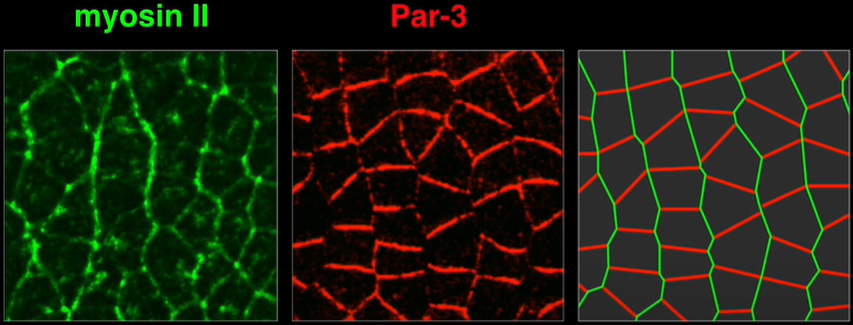
\includegraphics[width=\linewidth]{chapters/Theory/figures/bipolar-PCP.png}
    \end{subfigure}
    \caption{\cite{zallen2004patterned}\url{https://www.youtube.com/watch?v=MO7x7R-m3Qk}}
    
    \label{fig:ConvergentExtensionDiagram}
\end{figure}

Wieshaus and [hende damen der] showed through laser ablation, Cell Intecolation. Anisotropic constriction of cell borders with deformations only happening  



We know that the signaling protein Wnt plays an important role in controlling Convergent Extension. For interesting writing, here is some foreshadowing: Wnt is also known as an inducer of Planar-Cell-Polarity.

\subsection{ Apical Constriction }
When the cell sheet wants out-of-plane bending, they turn to Apical Constriction. Apical constriction functions exactly as you would think; Myosin rings constrict the apical (outer) side of the cell, creating a smaller surface area. This leads to bending and, when enough constriction is applied, invagination. (see Figure \ref{fig:apical-constriction}). Cells has been shown the ability to constrict both isotropically and anisotropically.

\begin{figure}[H]
    \centering
    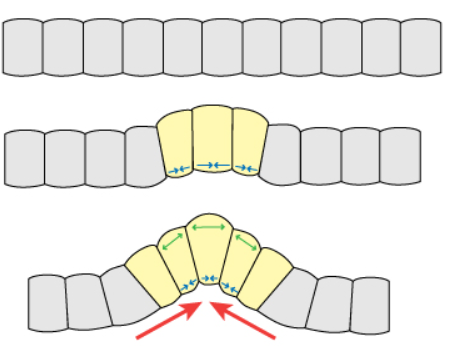
\includegraphics[width=0.3\linewidth]{chapters/Theory/figures/apical_constriction_schematic.png}
    \caption{Schematic for how apical constriction works}
    \label{fig:apical-constriction}
\end{figure}


\subsection{Cell Shape Change}
If each part is long, the total is long. This one is self-evident.
\subsection{Proliferation}
If cells are dividing in-plane, they can apply a pressure. In the stages of we are looking at, cell-division shown to not be a driving force.


\section{Drosophila Gastrulation in detail}
Now, with the details in place, we can get to the main event!
In 1975 Bownes et al. split the development of the fruit fly from fertilised egg to hatched larvae into 17 distinct events. \cite{bownes1975photographic} We will be looking at stages 5 through 7, lasting about 15 minutes. These are characterized by having the first mesoscopic morphogenetic movements and setting the stage for all the morphology to come. 

The Drosophila morphogenesis consist of a series of interconnected localized cell movements. I will here present an abridged (The "Good Parts" Version) overview, roughly ordered in time:
\newpage

\begin{figure}[H]
    \centering
    \vspace*{-1cm}\makebox[\textwidth]{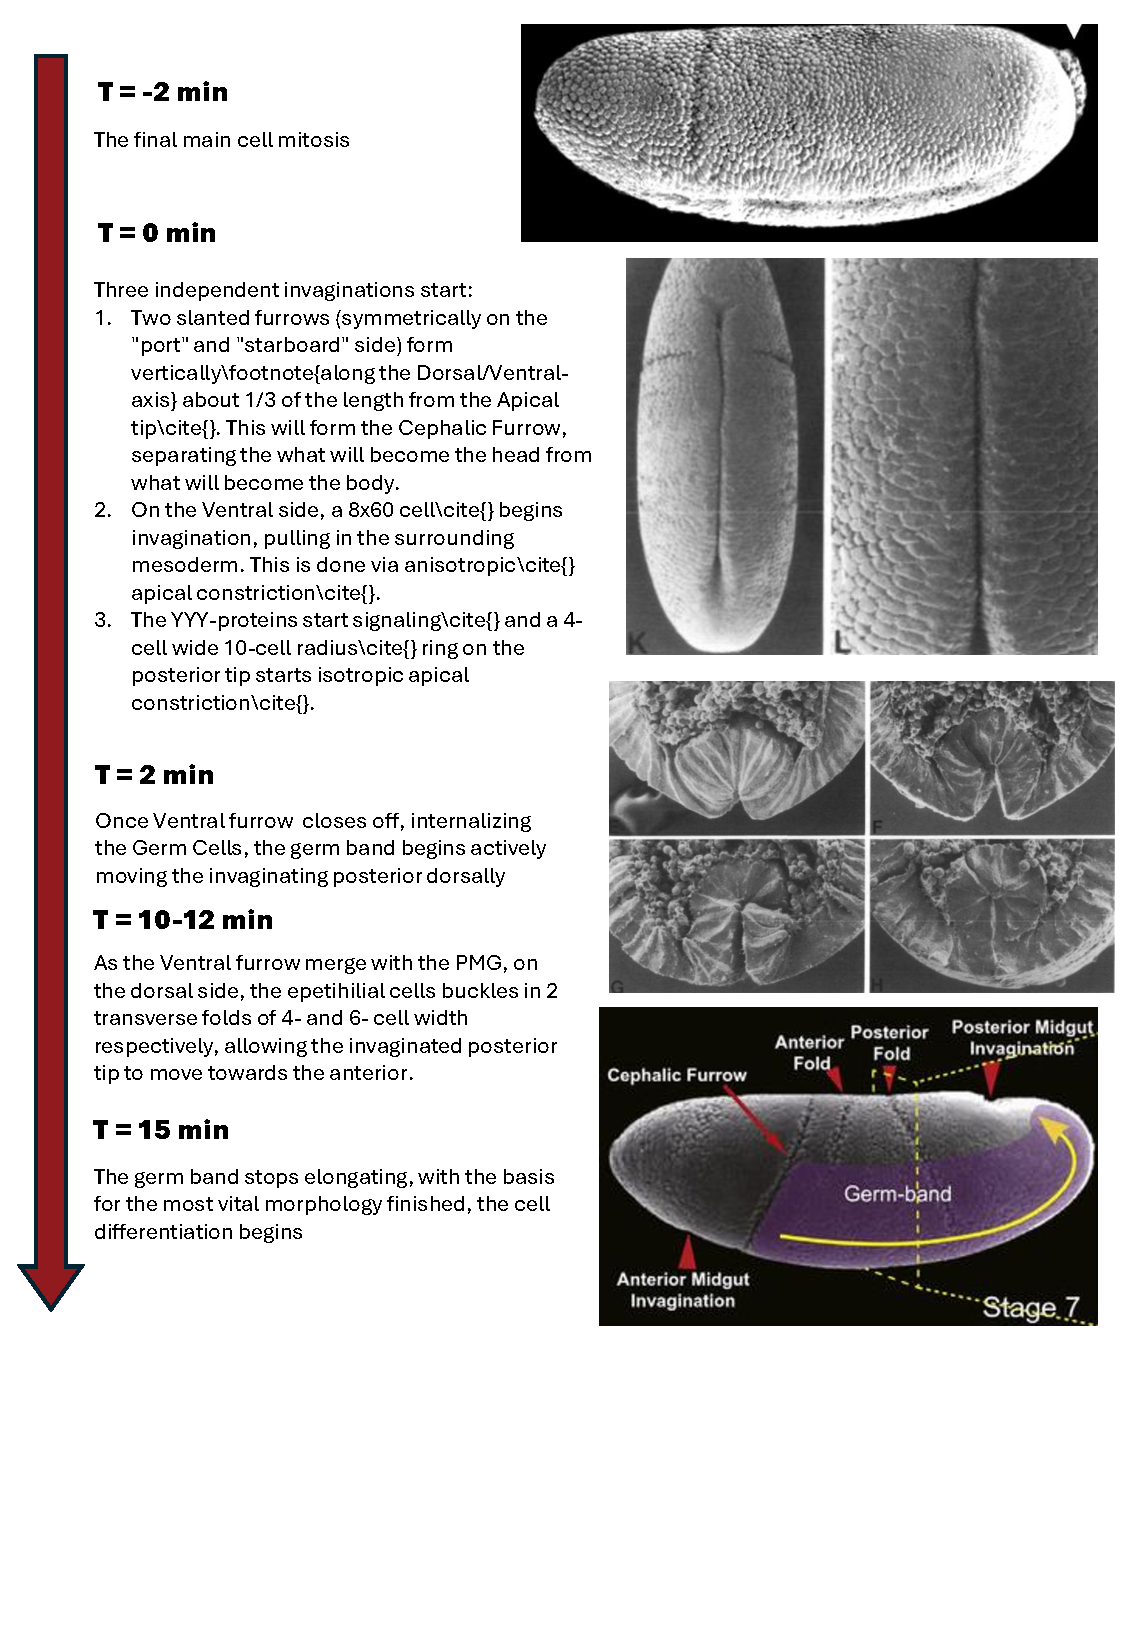
\includegraphics[width=0.8\paperwidth]{chapters/Theory/figures/Timeline.pdf}}
    \caption{Caption}
    \label{fig:enter-label}
\end{figure}
\newpage

\section{Previous attempts at simulation?}
While in silico models has provided multiple working examples of all the aforementioned embryogenesis events, their interplay has proven hard to study.

Mainly finite-element simulations have dominated the field when studying the physics of tubologenesis, tissue-folding etc.  


\section{Our Model}
This all leads us to to our:


The model is built around simply simulating the movement of the center of mass of the cells aling with their individual orientations. The principal [idea] is to elevate the Apical-Basal and Planar-Cell polarities by seeing them as explicitly stated polarization-vectors with mechanotransduction (as described in section \ref{sec:theory-polarity})

As described in \cite{} and \cite{}, the model we have been working with has the following intercellular potential:

\begin{equation}
    V_{ij}=e^{-r_{ij}}-A_{ij}e^{-r_{ij}/\beta}
\end{equation}

Where the quantity 
\begin{equation}
    U_i = \sum_j V_{ij}
\end{equation}
Where the sum is over all Line of sight/Voronoi neighbors (biologically founded if you remember the nearest neighbor protein connections in Figure \ref{fig:mysosinMeshwork})

For $A_{ij}=1$, the potential simply looks akin to a Yukawa/YYY potential and can be seen in Figure \ref{fig:potential} 
\begin{figure}[H]
    \centering
    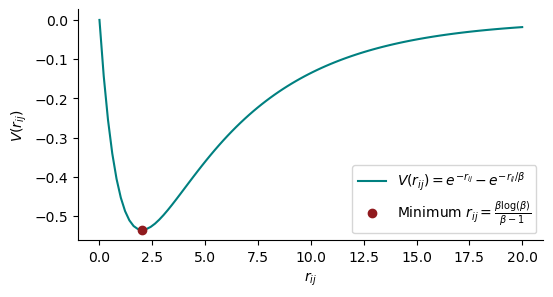
\includegraphics[width=0.7\linewidth]{chapters/Theory/figures/potential.png}
    \caption{The potential well our point particles lie in, with the minimum (ie. effective cell size) drawn in.}
    \label{fig:potential}
\end{figure}

$\cdots$


 introducing a more complicated parameter, 
\begin{equation}
    A_{ij}=\sum_{n=1}^{3}\lambda_n A_n
\end{equation}
where we sometimes keep the constraint $\sum_{n=1}^{3}\lambda_n=1$ but more often t


Taking inspiration from the previous sections about YYY we introduce the two biologically founded polarities: Apical-Basal (ie. inside/outside) and Planar Cell Polarity. ABP and PCP from here on. As previously mentioned in Section \ref{sec:gen_patterns}, the interplay between cell-polarisation and physical orientation goes both ways. This motivates the following three terms which I will quickly explain one by one:
\begin{subequations}
\begin{align}
S_1&=\left(\hat{p}_i \times \hat{r}_{i j}\right) \cdot\left(\hat{p}_j \times \hat{r}_{i j}\right)\label{eq:s1}\\
S_2&=\left(\hat{p}_i \times \hat{q}_{i}\right) \cdot\left(\hat{p}_j \times \hat{q}_{j}\right)\label{eq:s2}\\
S_3&=\left(\hat{q}_i \times \hat{r}_{i j}\right) \cdot\left(\hat{q}_j \times \hat{r}_{i j}\right)\label{eq:s3}
\end{align}
\end{subequations}



Trying to reference Equation \ref{eq:s2}

Now, having a potential defined, each timestep the cells move as subjects to overdamped dynamics:

\begin{equation}
    \frac{d \bar{x}_i}{d t}=-\frac{d V_i}{d \bar{x}_i}+\eta \hspace{1.5cm}|\hspace{1.5cm}  \bar{x} \in \{\bar{r}, \bar{p}, \bar{q}\}
\end{equation}

where $\eta$ is uncorrelated Gaussian noise.

The gradient is calculated via an automatic differentiation engine\footnote{The PyTorch-framework specifically} and the simulation time steps are calculated via Euler integration.


A number of modifications where added:
\begin{itemize}
    \item Preferential adhesion
    \item Nematic l1
    
\end{itemize}


For notes on the actual implementation see Section \ref{App:Code} in the Appendix.


\chapter{Results}
\label{chap:res}
\section{List of model features/parameters and their biological foundation}
\section{Visual closeness}
\subsection{Ventral Furrow}
After mitosis stops, the the first visual change on the is the belly, where a distinct cleft begins forming. \\

While all cells expressing \textit{twist} \& \textit{snail} lower their apical surface area, they do not constrict indiscriminately, instead starting with the \textit{inner} 8x60 cells.[citation needed] As the furrow closes off, creating closed-off tube with a recognizable light bulb-shape in the cross section, the invaginated tissue "disconnects". This was not part of our simulation.

In figure \ref{fig:VFComparison}, a comparison between

\begin{figure}[H]
    \centering
    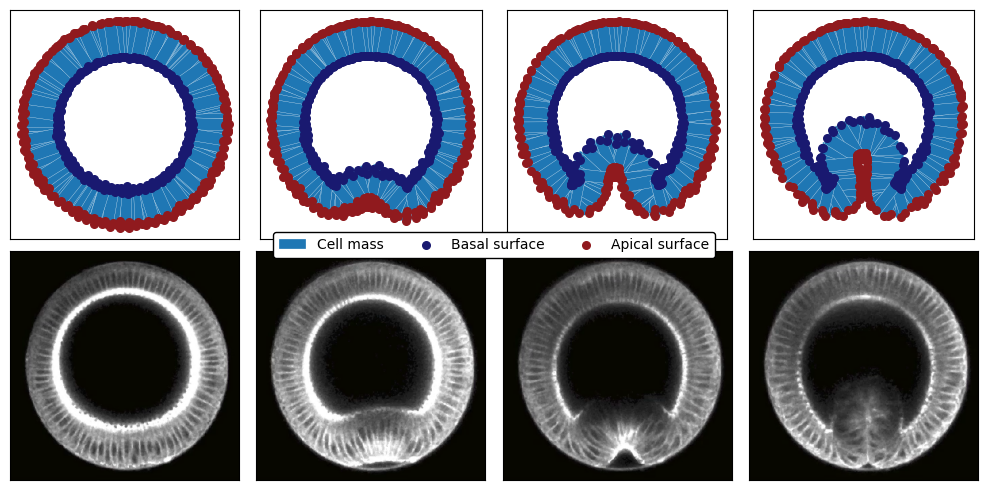
\includegraphics[width=1\linewidth]{chapters/Results/figures/VF_comparison.png}
    \caption{A comparison of simulation and frames from live development. \textbf{Upper row}: Simulation. \textbf{Lower row}: Multi-photon microscopy. \\Each frame is taken at equally spaced time intervals. Cross section video borrowed from \cite{conte2012biomechanical}}
    \label{fig:VFComparison}
\end{figure}


Maybe quantify here?
I am guessing we can do a cell-center fit?
Out of scope? Yes. Would be cool? Also yes.
\subsection{Germ band}
The Germ Band is defined as.

Seeing hwo 

\begin{figure}[H]
    \centering
    \begin{subfigure}[b]{0.25\textwidth}
        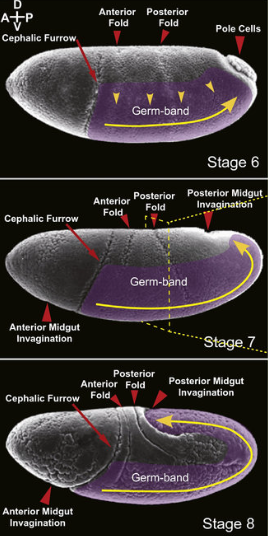
\includegraphics[width=\textwidth]{chapters/Results/figures/compareGB.png}
    \caption{Figure from\cite{kong2017forces} }
        
    \end{subfigure}
     \hfill
    \begin{subfigure}[b]{0.7\textwidth}
    
\includegraphics[width=\textwidth]{chapters/Results/figures/gb_firstframe_lastframe.png}
    \caption{Colored in germ band. Elongating posteriorly, moving ventrally.}
    \end{subfigure}
    
\end{figure}


Lorem ipsum dolor 
\\

The individual movements:

\begin{figure}[H]
    \centering
    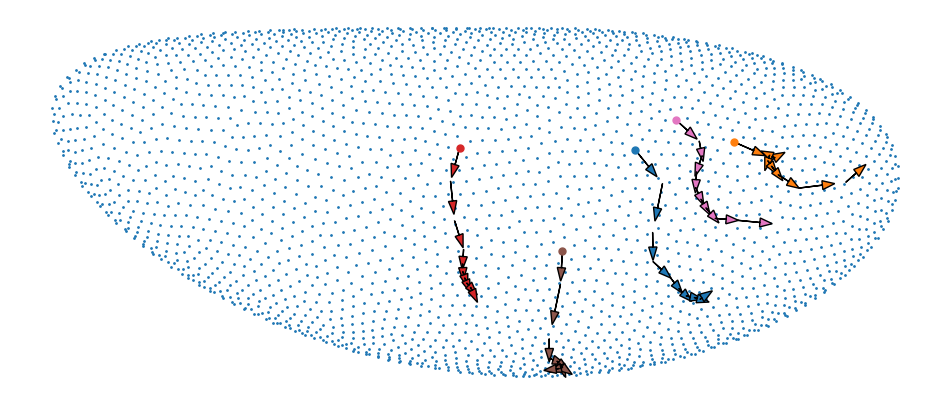
\includegraphics[width=1\linewidth]{chapters/Results/figures/movements.png}
    \caption{NOT TO SELF: Remove some of the cells -- it's cluttered!}
    \label{fig:enter-label}
\end{figure}


\begin{figure}[H]
    \centering
    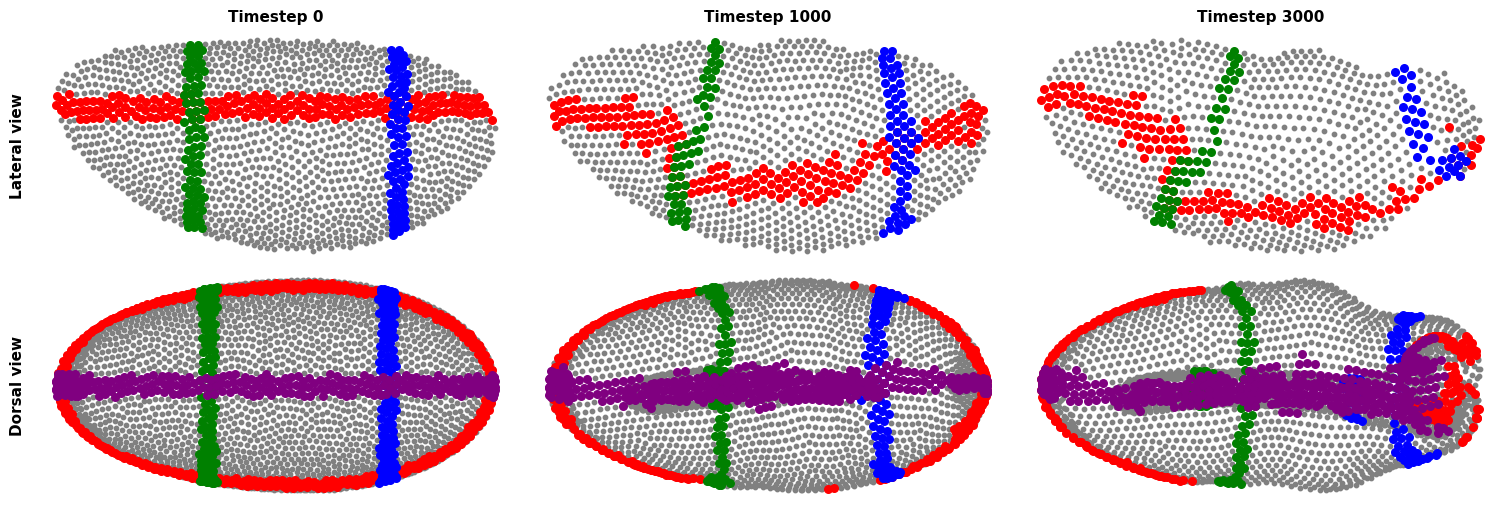
\includegraphics[width=1\linewidth]{chapters/Results/figures/band_movements.png}
    \caption{My simulation. Compare to figure \ref{fig:band-movements-stas}}
    \label{fig:band-movements}
\end{figure}
\begin{figure}[H]
    \centering
    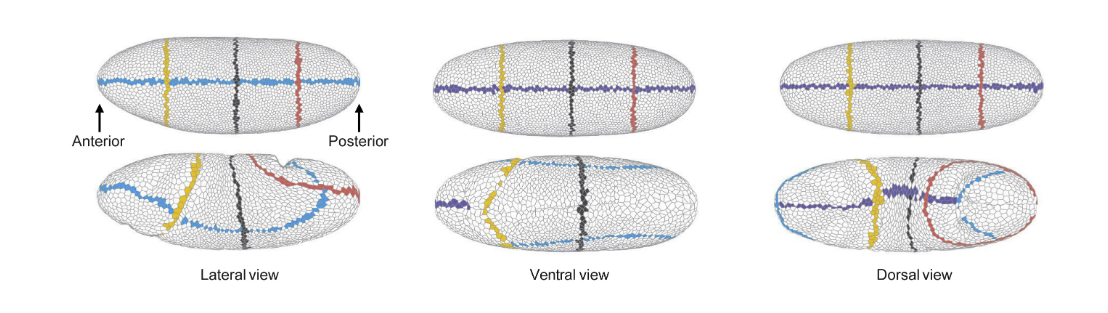
\includegraphics[width=1\linewidth]{chapters/Results/figures/compareStasGBShape.png}
    \caption{Coloured segmented images. Taken from from the brilliant\cite{stern2022deconstructing}. Compare to figure \ref{fig:band-movements}. NOTE TO SELF: Cut only important parts out}
    \label{fig:band-movements-stas}
\end{figure}

% \subsection{Auxiliary furrows}
\subsection{Daniel}
\section{Quantitative closeness}
\subsection{Movements}

\begin{figure}[H]
    \centering
    \makebox[\textwidth][c]{
    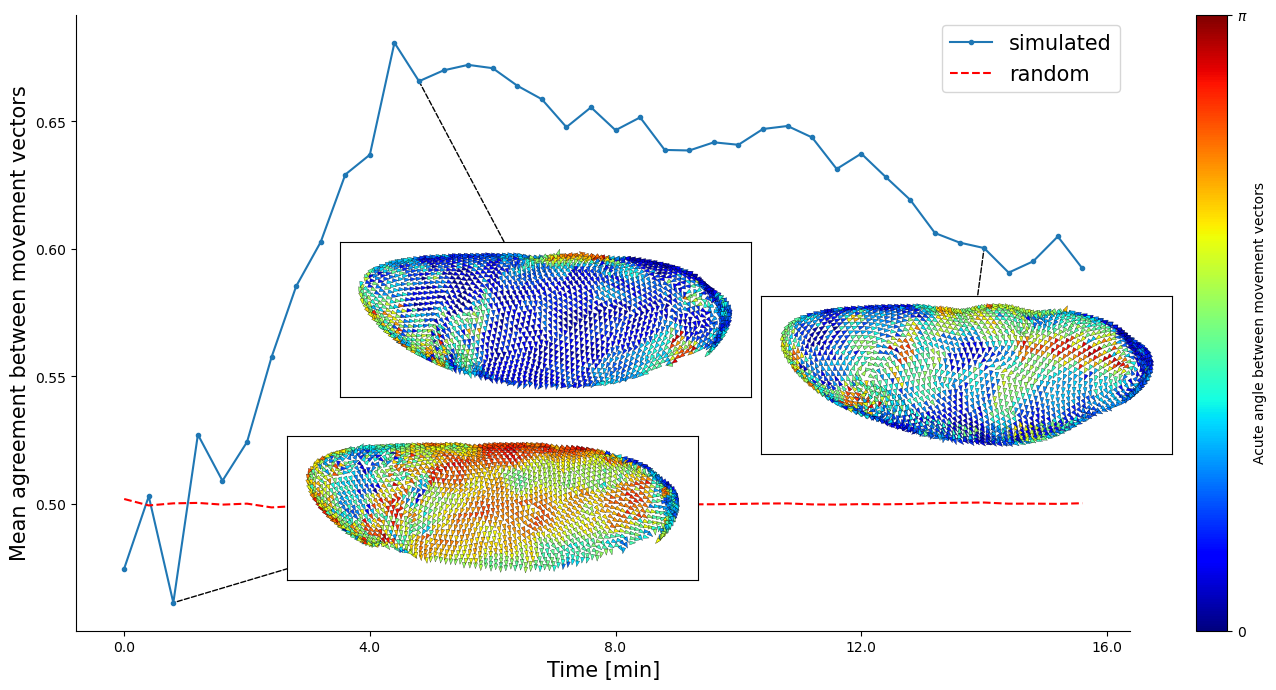
\includegraphics[width=1.3\linewidth]{chapters/Results/figures/movement_vectors_normal.png}
    }
    \caption{Caption}
    \label{fig:enter-label}
\end{figure}

\subsection{Timing}
Even though cells have been shown to have remarkably precise internal clocks\footnote{cool footnote with a remarkable number}\cite{}, there is no evidence for any specific timing in stages 5-7 [citation needed].\textbf{ This is a main result} The fact that we have recapitulated(?) much of the dynamics completely without any explicit time-dependent parameters seems to corroborate our thesis proposed in Section \ref{sec:timedependence}, that Boundary Conditions, Initial Conditions and an inter-atomic rule-set is sufficient for arbitrarily complex morphology/anatomy to arise.\footnote{A sort of Curtis–Hedlund–Lyndon theorem for cells}    

This might be a result of real time 'global' information sharing being limited and not jsut reactions to maternal morphogens.

There is also the "biological clock"\cite{johanolsen2} that proteins themselves have dynamic structure that can change over time.\cite{johanolsen1}
\subsection{Strain}

\subsection{Rosettes}
\begin{figure}[H]
    \centering
    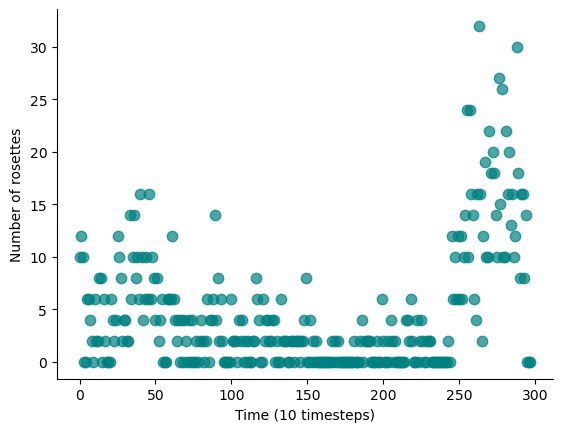
\includegraphics[width=0.5\linewidth]{chapters/Results/figures/rosettes_time.png}
    \caption{Caption}
    \label{fig:enter-label}
\end{figure}

\subsection{Daniel-data?}
\newpage
\section{In Silico Mutant "predictions" - compared to phenotypes and reference model}
\subsection{No PMG}

Knocking out \dots

\begin{figure}[H]
    \centering
    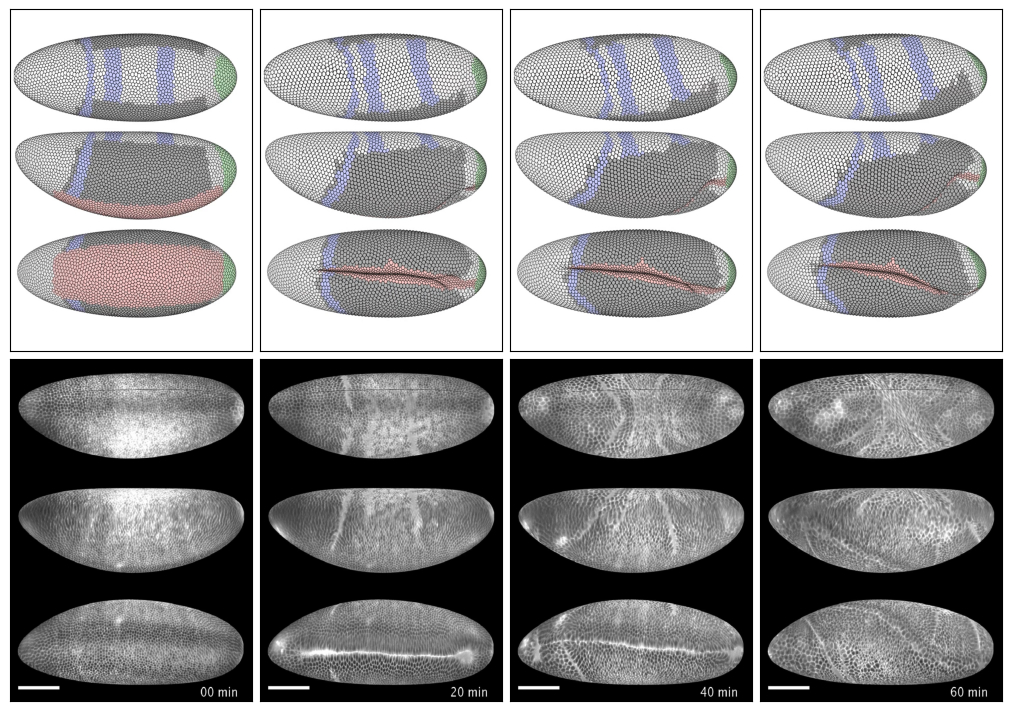
\includegraphics[width=1\linewidth]{chapters/Results/figures/corkscrew_comparison.png}
    \caption{Comparing the \textit{Corkscrew} phenotype with my simulation. Video taken from \cite{smits2023maintaining}}
    \label{fig:corkscrew-comparison}
\end{figure}
% Twist and shout
\subsection{No Ventral Furrow}
% \url{https://genesdev.cshlp.org/content/5/9/1568.full.pdf}
% We are seeing the right thing
\subsection{No Cephalic Furrow?}
% maybe not important
\subsection{No active intercolation / Germ band}
% \url{https://softmath.seas.harvard.edu/wp-content/uploads/2019/10/2009-07.pdf}
% clear that model is missing cell shape change!
\section{Additive/subtractive working together matrix}
% \subsubsection{}


\chapter{Conclusion}
\label{chap:con}
\section{Questions}
\todo{Give me all the questions again}
Q0 - Mimimal umber of rules for vivo-like gastrulation to emerge\\
Q1 - Are BC/IC sufficient?\\
Q2 - Given a bottom-up, full scale model, what can we say re: domain-interactions\\
\\\\
Result 1: Visual and quantitative comparison between Silico and Vivo\\
Result 2a: Comparison between Silico mutants and Vivo mutants\\
Result 2a: Comparison between Silico mutants and Silico optimal (remember to include PCP-orientation)\\

\section{Answers}
\begin{itemize}
    \item Polarizations and cell-interactions only set from biologically founded initial conditions.
    \item No explicit timing
    \item No chemotaxis
    \item No large-scale "information sharing"
    \item Stable under perturbations
    \item With a p-value of 
\end{itemize}

While looking at the [small parts] in many cases can lead to crudely reductionist conclusions, 

We have seen that even if many biological systems are "more than than the sum of its parts", having a model for the parts can allow for .

We have shown that complex time-[something] of events can arise from the physically simple interactions with boundary conditions and mechanical feedback-loops.



\textbf{Comparisons to data}\\
We have found through multiple comparisons, how our simulation is recapitulating the dynamics.

The movement vectors, timing, strain-distribution over time and rosettes all had clear relations[?] to reality while also showing the different shortcomings where our methodology could be improved.
\textbf{Further work}

We have identified the possibility of cell shape change (i.e. anisotropic relaxation distances in relation to external pressure) to be the most promising next step. Some work was already put into this witout anything fruitful. Other potential expansions on the model would be for the dorsal and cephalic folds to buckle under pressure. Also adding in the in-plane proliferation in the cephalic region. This was implemented, but removed for simplicity.

\textbf{Combinations}
We have seen that every part of the simulated embryo was necessary for successful gastrulation. 
While both our model and nature is stable to noise and YYY, the enviroment, boundary conditions and initial conditions are vital for defining YYY

\textbf{closing remarks}
Turing showed that simple interplay between chemicals can create arbitrarily complex biopatterning that can serve as a blueprint. We have taken a step in the direction of showing how a combination between minimal environmental information and simple rules for the interplay between individual cells can lead to the creation of physical form. \todo{rephrase}


% \chapter{Outlook}
% \label{chap:out}
% The British Mathematician George Box is often quoted for saying \textit{"All models are wrong. Some models are useful"}. 

We have a minimum, wholly biologically founded model. It is not as stable as mother nature, .

This is my model. There are many like it, but this one is mine.



% List of publications: The title appears as large as a Chapter header in the document, but as large as a section in the table of Contents, and there are no more page headers.



\addcontentsline{toc}{chapter}{Bibliography}
\bibliography{references}

\appendix
\renewcommand{\thesection}{A\arabic{section}}
\addcontentsline{toc}{chapter}{Appendix}
\chapter*{Appendix}
\section{Unused plots}
\label{App:Plots}
\begin{figure}[H]
    \centering
    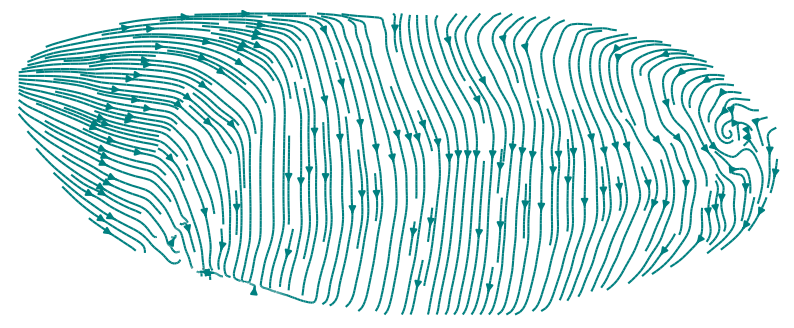
\includegraphics[width=1\linewidth]{chapters/Appendix/streamplot1.png}
\end{figure}


\begin{figure}[H]
    \centering
    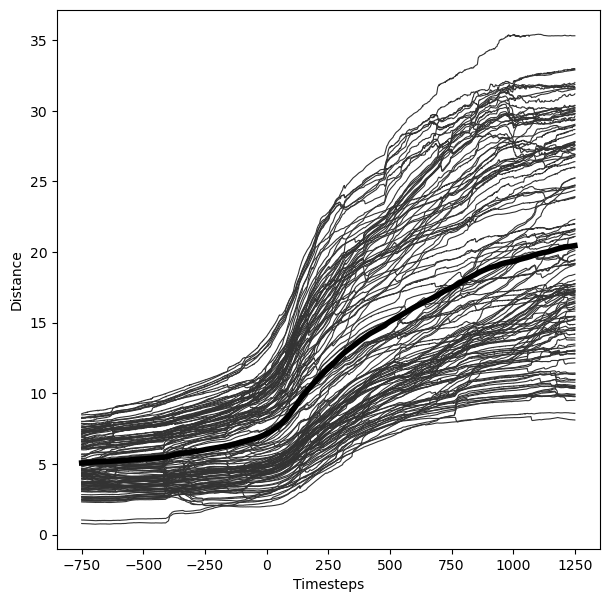
\includegraphics[width=1\linewidth]{chapters/Appendix/germbandMovementQuant.png}
    \caption{Horizontal-position of a line of germ-band cells, mirroring the analysis in  \url{https://www.ncbi.nlm.nih.gov/pmc/articles/PMC2801059/}}
    \label{fig:enter-label}
\end{figure}
\begin{figure}[H]
    \centering
    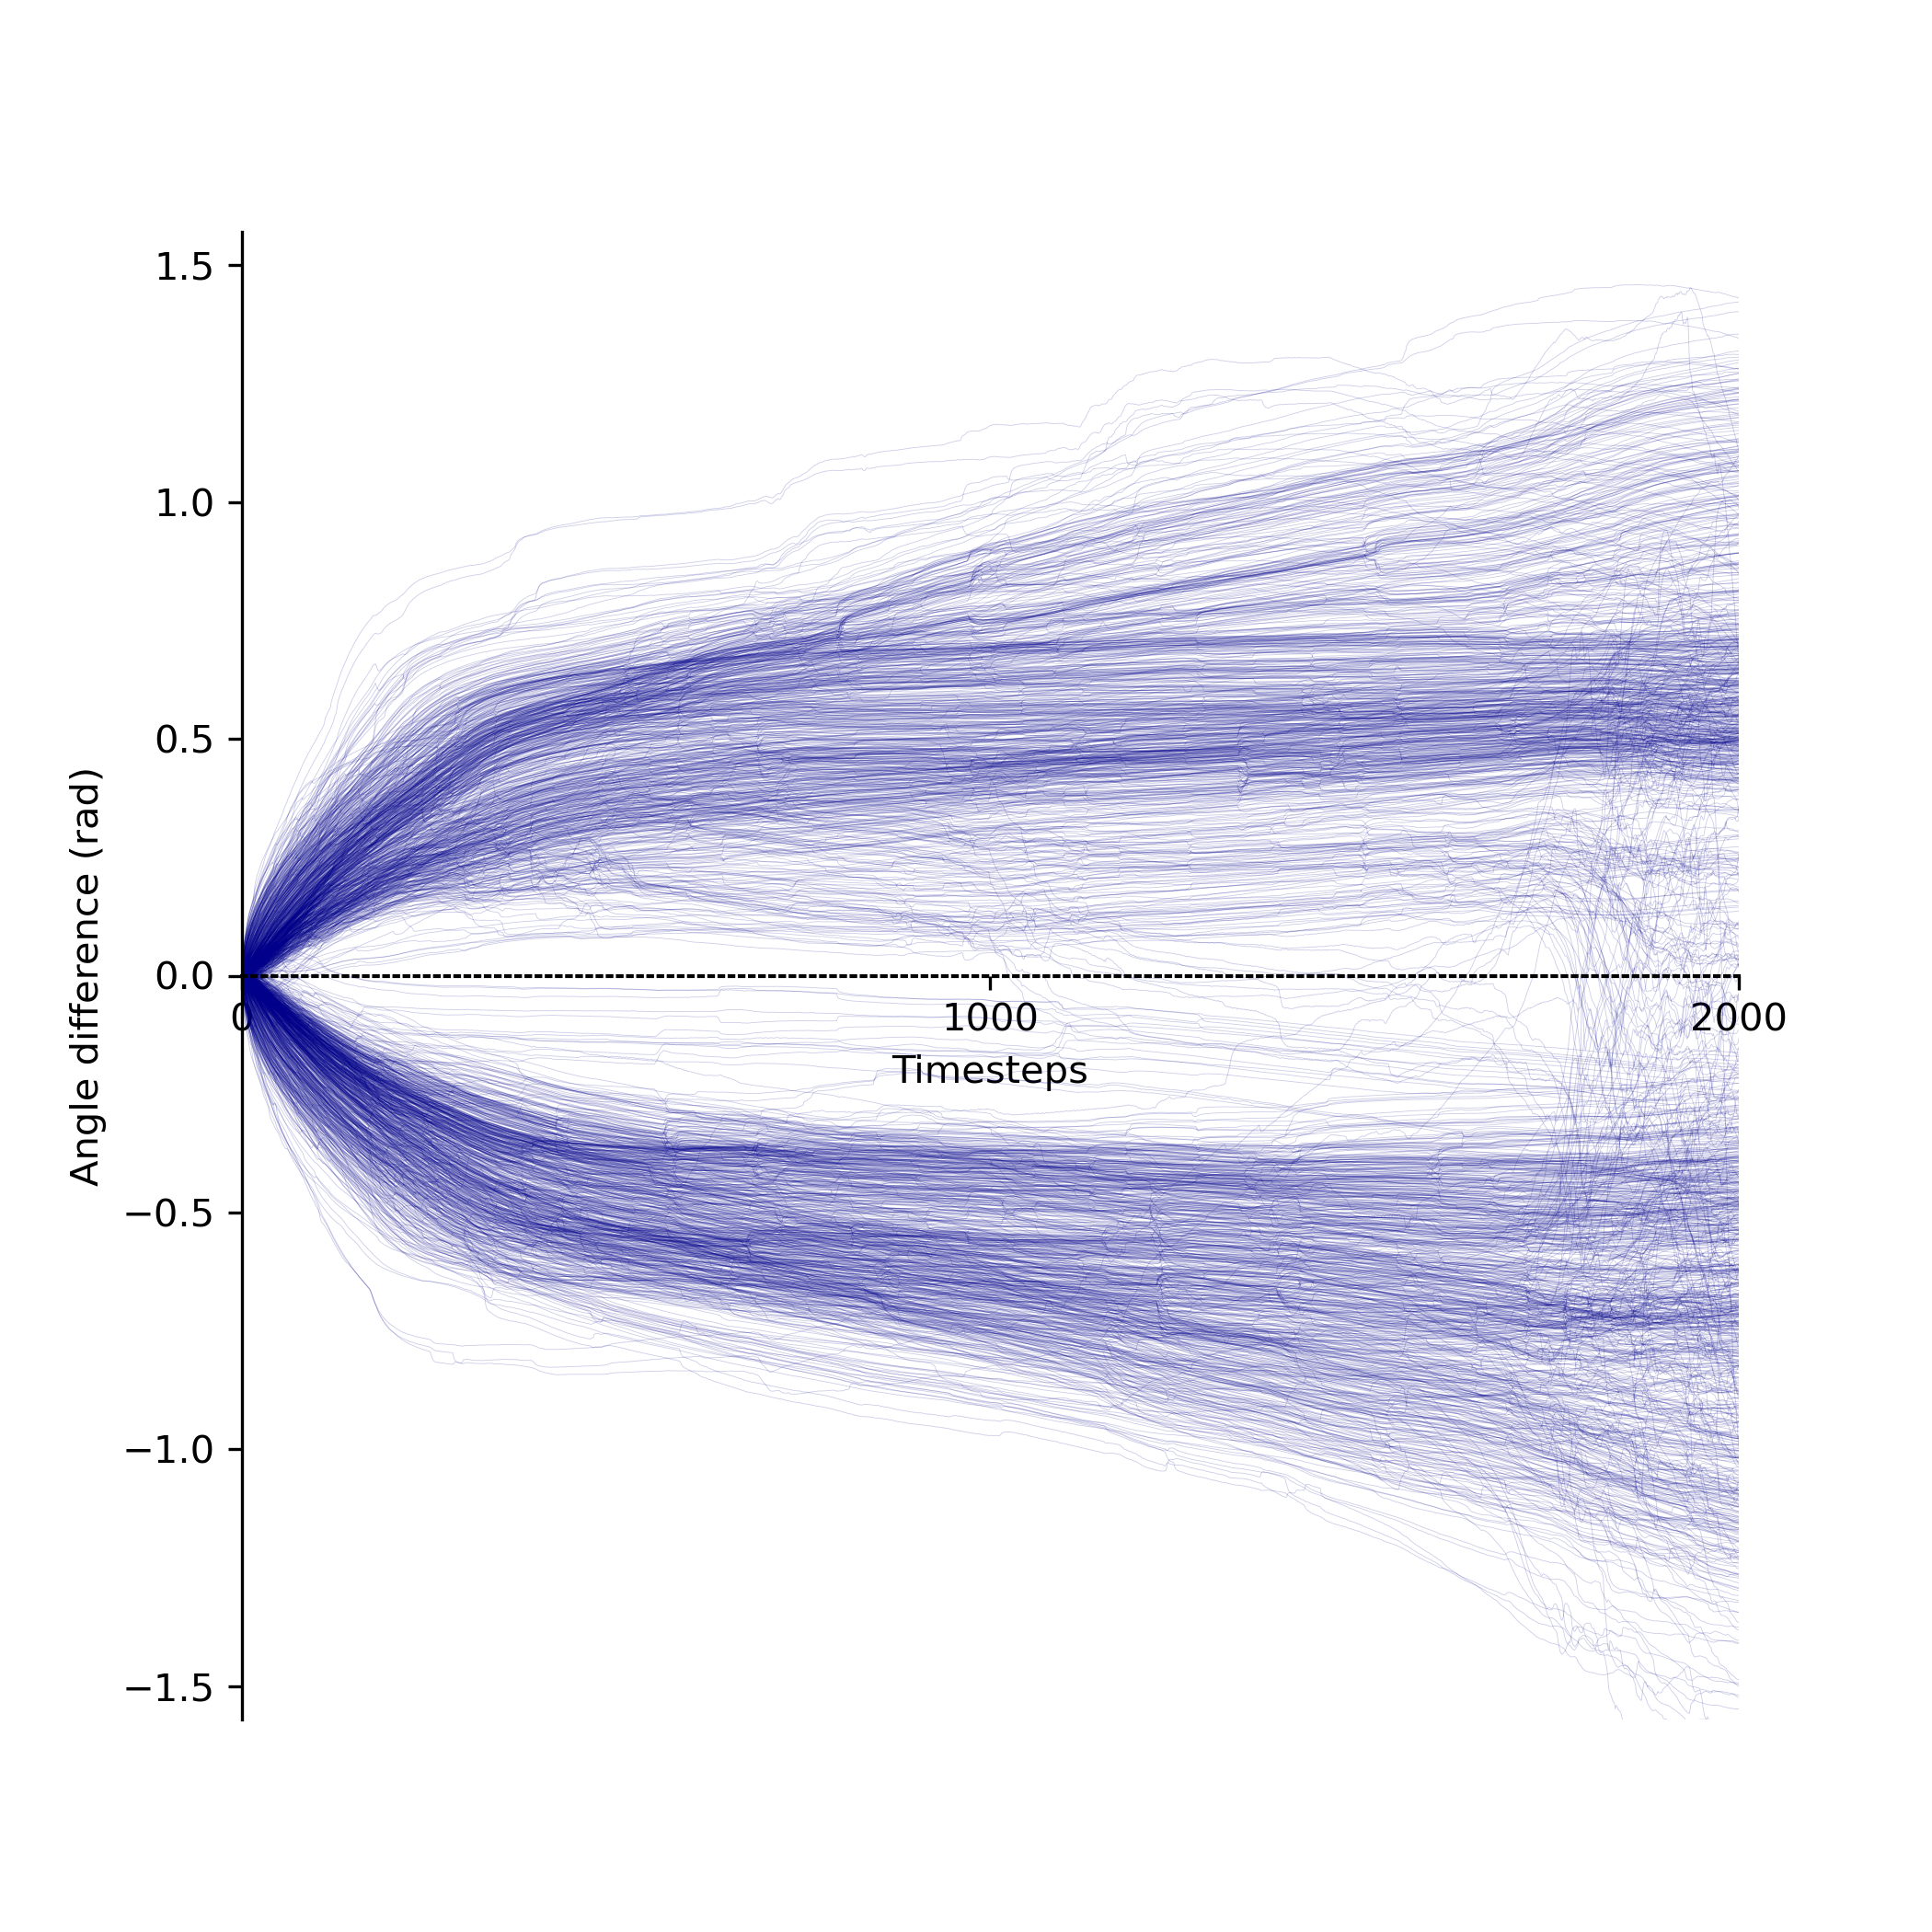
\includegraphics[width=1\linewidth]{chapters/Appendix/the_ring.png}
    \caption{Angle in cylindrical coordinates of germ-band. Mirroring \url{https://www.ncbi.nlm.nih.gov/pmc/articles/PMC2801059/}}
    \label{fig:enter-label}
\end{figure}
\section{Code details}
\label{App:Code}
\section{Additional Videos}
\label{App:videos}
\section{Sergei-analyses (tie into PCP)}
\label{App:Sergei}
\section{Green-Lagrange strain inference}
\label{App:Strain-Calculation}
Firstly transform into cylindrical coordinates.... \\
"A strain rate is the ratio of the change in length to the original length, divided by the time interval, with units of proportion (pp) per minute. The lines show the mean strain rates for all five embryos, and the ribbon width represents the average standard error within a data set. The timing of developmental landmarks is shown for the five embryos recorded"\cite{butler2009cell}
\section{Why our rosettes behave differntly }
\label{App:why-rosettes}
In our model, where the equilibrium distance is the same for every direction no matter the pressure exerted, getting a bimodality is predictable.
Every time a new pair 'touch' on the up-down axis, they release space for a pair above or below on the perpendicular axis. 


\section{We have not taking the following into account}
\subsection*{Cell shape change!}
\subsection*{Mitotic pressure in cephalic area}
\subsection*{Things that change over time}
\subsection*{Pressure-buckling of dorsal folds}
\subsection*{Pressure from yolk}
\section{Detailed morphogens}
\label{App:morphogens}
\begin{table}[H]
\begin{tabular}{lll}
 \begin{tabular}[c]{@{}l@{}}Genetically patterned \\ transcription factor proteins\end{tabular} & Location at gastrulation & Vital for development of \\ \hline
 Twist \& Snail                                                                                 & Ventral                  & Mesoderm                 \\
Huckebein \& Tailless                                                                          & Posterior                & Endoderm (Midgut)   \\

 Runt \& Even skipped & Germ Band & All of the above\\
Buttonhead \& Even skipped  & Cephalic furrow & Chephalic furrow\\

\end{tabular}
    \caption{The most important morphogens and their simplified reason of significance}
    \label{tab:morphogens}
\end{table}


\begin{lstlisting}
# The germ band requires striping to be active [citation]
GB = GE.or_gene(GE.gene("eve"), GE.gene("run"))

# A cutoff was needed because of spotty coverage
# As can be seen on all, the germ-band does not extend far up
# we expect some inhibiting gene to be doing this IRL
GB[GE.base[:,2] > 50] = 0

# remove in the head domain
GB = GE.not_gene(GB, GE.gene("fkh"))

# ...
GE.add_expression(GE.get_second_run_stripe(), 0.4, True, 5)  # Second Run Stripe

GE.add_expression(GE.get_fifth_run_stripe(), 0.4, True, 5)  # Second Run Stripe

GE.add_expression(GB, 0.2, True, 1)  # Germ Band

# GE.add_expression(GE.not_gene(GE.or_gene(GE.gene("eve"), GE.gene("run")), GE.gene("Doc2")), 0.2, True, 1)  # Germ Band

GE.add_expression(GE.gene("Dfd"), 0.6, True, 5)  # Cephalic Furrow


# GE.add_expression(GE.not_gene(GE.and_gene(GE.gene("Kr"),GE.gene("run")), GE.gene("sna")), 0.2, True, 5)  # posterior fold

twi = GE.gene("twi")

twi[GE.base[:,1] > 25] = 0.
twi[GE.base[:,1] < -25] = 0.

# GE.add_expression(twi, 0.3, True, 4)  # Ventral Furrow (Daniel)


twist_and_snail = GE.and_gene(GE.gene("twi"), GE.gene("sna"))

# twist_and_snail[GE.base[:,0] > 140] = 0.

GE.add_expression(twist_and_snail, 0.2, True, 2)  # Ventral Furrow


GE.add_expression(GE.gene("hkb"), 0.25, True, 4)  # PMG
# GE.add_expression(GE.gene("hkb",), 0.6, True, 3)


GE.add_expression(GE.or_gene(GE.gene("croc"), GE.gene("oc")), 0.4, True, 0)  # Invert


GE.save("no_q_from_runt", q_from_runt=False)
\end{lstlisting}

\subsubsection{Cell types extracted from data}
When we say that the cell types were extracted from data, this comes with a couple asterisks:\\
Any expression in the cephalic region was removed by hand.\\
\textbf{Cephalic furrow}
In the data-set there were no [Cephalic furrow gene], but using the website [website] we could see that it spatially coincided with [other gene] which was in the data-set and was therefore used as a proxy. 
\textbf{Germ-band}
The germ-band was cut off by hand as the [gene1] and [gene2] expressions were very spotty at the top and the germ-band would not extend correctly.\footnote{I am guessing a suppressing gene that we did not take into account is also at play} 

\textbf{Ventral furrow}
Even though all the cells expressing \textit{twist} \& \textit{snail} on the belly lower their apical surface area, they do not constrict indiscriminately. Instead they start out by constricting in the \textit{inner} 8x60 cells. [citation needed] It is believed to be a more stable way of wedging [citation needed] but is still strange and not fully understood. [citation needed]. This meant that a specific rule for the wedging in the ventral region was needed. The inner 8 cells has a wedging constant $\alpha = 0.5$ while the rest has $\alpha = 0.2$.

\section*{Rosette analysis}
Convergent Extension is seen as a vital part of the development of many different YYY. Therefore multiple different methods of analysis and YYY have been developed.
One of the main quantifiers consist of looking at a cluster of neighboring cells that undergo convergent extension. These clusters are called Rosettes. Trough laser-ablation is has been shown that the Rosettes (as shown in the diagram on Figure \ref{fig:ConvergentExtensionDiagram}) can consist of up two twelve internally connected cells [citation needed].
For drosophila gastrulation in particular, the direction between each newly acquired neighbor is \todo{finish thought}



% \begin{figure}[H]
%     \centering
%     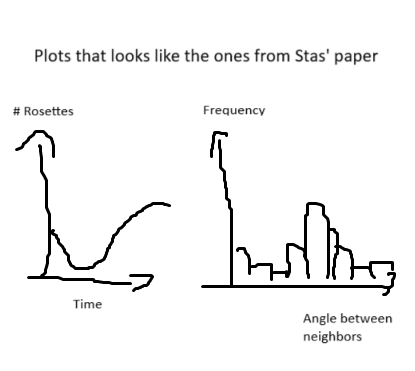
\includegraphics[width=0.8\linewidth]{chapters/Results/figures/rosettes_placeholder.png}
%     \caption{Caption}
%     \label{fig:enter-label}
% \end{figure}


\begin{figure}[H]
    \centering
    \makebox[\textwidth][c]{
    \begin{subfigure}[b]{0.55\textwidth}
    \centering
        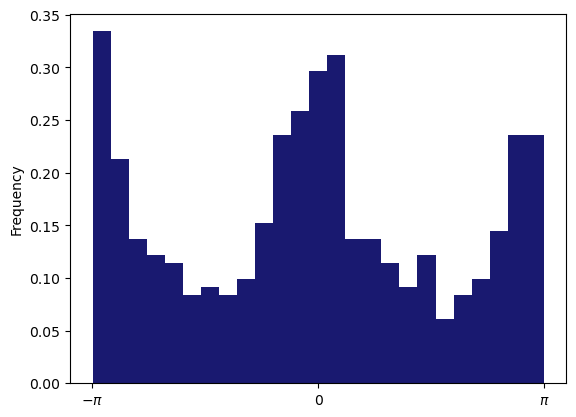
\includegraphics[width=\linewidth]{chapters/Results/figures/rosettes_angle_dist.png}

    \end{subfigure}
    \begin{subfigure}[b]{0.5\textwidth}
    \centering
    
    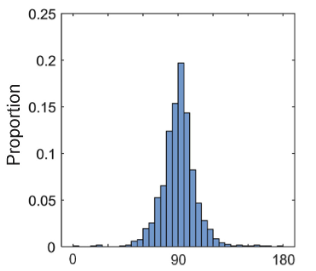
\includegraphics[width=\linewidth]{chapters/Results/figures/rosettes_angle_dist_data.png}
    \end{subfigure}
    }
    \caption{The angular distribution of the newly acquired neighbors in rosettes as found in (\textbf{left}) simulation (in radians) and (\textbf{right}) data (in degrees).}
    \label{fig:roestte-angle-dist}
    
\end{figure}
In Figure \ref{fig:roestte-angle-dist}, the distribution of angles of all found rosette-events can be seen. Strangely, the distribution is clearly bimodal in horizontal and vertical, where the ground truth has a single peak at the vertical axis. 

We believe the lack of malleability in the contours of the cells might be to blame.


% When speaking with Daniel, a researcher at the [Stas'] laboratory who did the original analysis, he said that this makes sense, as looking at neighboring nuclei is fundamentally different from edges. \todo{rephrase to make less bad}. 

% I won't bore you the details, so a quick run-down of our thoughts and discussions can be found in Section \ref{App:why-rosettes} in the Appendix.\\

% ... \\
% Speaking of Daniel:
\note{
Not showing something good :( Keep for completeness or move to appendix?}

% \subsection{Daniel-data?}
% Nothing here yet...
% \begin{figure}[H]
%     \centering
%     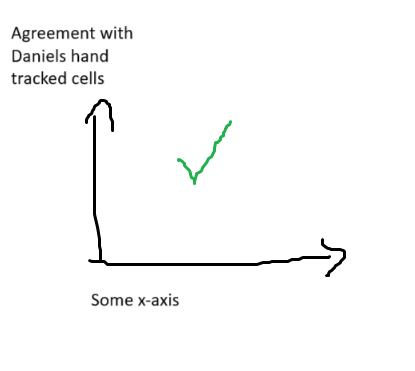
\includegraphics[width=0.7\linewidth]{chapters/Results/figures/daniel_placeholder.png}
%     \caption{Some caption}
%     \label{fig:enter-label}
% \end{figure}

\section*{Other efforts we have tried in vain}


\end{document}
